\documentclass{article}
\usepackage{amsmath, amssymb}
\usepackage{tikz}
\usetikzlibrary{decorations.markings}

\begin{document}

\begin{figure}[h]
    \centering
    \begin{tikzpicture}[scale=1]
        % Axes
        \draw[->] (-3.5, 0) -- (3, 0) node[right] {$\Re$};
        \draw[->] (0, -2.5) -- (0, 3) node[above] {$\Im$};

        % Contour $\Gamma_\lambda$
        \draw [thick, domain=0:90, variable=\t, samples=100] plot ({\t*0.75 + 2.25 * cos(\t)}, {2.25 * sin(\t)});
        \draw [thick, domain=90:180, variable=\t, samples=100] plot ({-2.25 * cos(\t)},{2.25 * sin(\t)});
        \draw [thick, domain=180:270, variable=\t, samples=100] plot ({-2.25 * cos(\t)},{-2.25 * sin(\t)});
        \draw [thick, domain=270:360, variable=\t, samples=100] plot ({\t*0.75 - 2.25 * cos(\t)}, {-2.25 * sin(\t)});

        % Dashed line
        \draw[thin, dashed, ->] (0,0) -- (0,2) node[midway, right] {$\sigma(T)$};
        \draw[thin, dashed, ->] (0,0) -- (2,0) node[midway, below] {$\kappa^2$};
        \draw[thin, dashed, ->] (0,0) -- (-1.75,0) node[midway, above] {$-\lambda/2$};

        % Labels
        \node at (3.2,1.5) {\small $\Gamma_\lambda$};
    \end{tikzpicture}
    \caption{An illustration of the contour $\Gamma_\lambda$ defined in \cref{eq:contour}. The region enclosed by $\Gamma_{\lambda}$ is just $D_\lambda$ in \cref{assu:Filter}. The dashed interval $[0,\kappa^2]$ contains the spectrum of $T$ and $T_X$.}
    \label{fig:contour}
\end{figure}

\end{document}